\documentclass[final]{beamer}

% ====================
% Пакеты (Ваш базовый набор + Beamerposter)
% ====================
\usepackage[T2A]{fontenc} % Корректная кодировка шрифтов для кириллицы
\usepackage[utf8]{inputenc}
\usepackage[english, russian]{babel} % Поддержка двух языков

% Ваши математические и графические пакеты
\usepackage{amsmath}
\usepackage{amssymb}
\usepackage{graphicx}
\usepackage{multicol}
\usepackage{tikz}
\usepackage{float}
\usetikzlibrary{calc, intersections}
% Пакеты для оформления постера (A1, портретная ориентация)
\usepackage[size=a1,orientation=portrait,scale=1.12]{beamerposter}
\usetheme{gemini}
\usecolortheme{msu}
\usepackage{booktabs} % Оставляем для красивых таблиц (toprule/midrule)

% ====================
% Ваши макросы и сокращения
% ====================
\newcommand{\fr}{\frac}
\newcommand{\pd}{\partial}
\newcommand{\limm}{\lim\limits}
\newcommand{\vect}{\overline}
\newcommand{\divisible}{\;\mathop{\raisebox{-2pt}{\vdots}}\;}
\DeclareMathOperator{\sign}{sign}

% ====================
% Геометрия колонок (Разметка)
% ====================
\newlength{\sepwidth}
\newlength{\colwidth}
\setlength{\sepwidth}{0.025\paperwidth}
\setlength{\colwidth}{0.3\paperwidth}

\newcommand{\separatorcolumn}{\begin{column}{\sepwidth}\end{column}}

% ====================
% Информационная часть
% ====================
\title{Оптимизация с помощью LLM}
\author{Марин Кирилл, Останин Андрей}
\institute[МФТИ]{Московский физико-технический институт}

% Футер (Нижняя плашка)
\footercontent{
  \href{mailto:marin.kp@phystech.edu}{marin.kp@phystech.edu} \hfill
  Постерная сессия \hfill
  \href{mailto:ostanin.am@phystech.edu}{ostanin.am@phystech.edu}
}

% Логотип (Если файлов нет, закомментируйте эту строку)
\logoright{
\includegraphics[height=6cm]{images/mipt_rus_inv_eps.pdf}}

% ====================
% Документ
% ====================
\begin{document}

\begin{frame}[t]
\begin{columns}[t]
\separatorcolumn

% --- КОЛОНКА 1 ---
\begin{column}{\colwidth}

  \begin{block}{Discrete Neural algorithmic reasoning}
    Архитектура воспроизводит пошаговое выполнение алгоритмов на графах помощью механизмов hard graph attention \cite{rodionov2025discreteneuralalgorithmicreasoning}. С учётом того, что любое представление входных данных может быть сведено к графовому виду, модель легко применяется к любой алгоритмической задаче. 

    Преимущество модели по отношению к обычным методам состоит в том, что архитектура не чувствительна к размерности задачи, что даёт возможность проводить обучение на задачах меньшей размерности и проводить inference за полиномиальное время в силу устройства архитектуры.
  \end{block}

  % РАЗДЕЛЕНИЕ НА ДВЕ МИНИ-КОЛОНКИ (БЕЗ использования block внутри minipage)
  \begin{block}{Эксперименты и задачи}
    {\large \textbf{Графовые задачи}}
    \vspace{0.5cm}

    В процессе исследования рассмотрено применение архитектуры к задаче поиска кратчайшего пути, а именно посредством воспроизведения алгоритма Дийкстры.
    \vspace{0.5cm}

    \begin{center}
      \begin{tabular}{lr}
        \toprule
        pointer\_accuracy & 1.0 \\
        pointer\_accuracy\_graph\_level & 1.0 \\
        \bottomrule
      \end{tabular}
    \end{center}
    \vspace{0.5cm}

    \begin{center}
      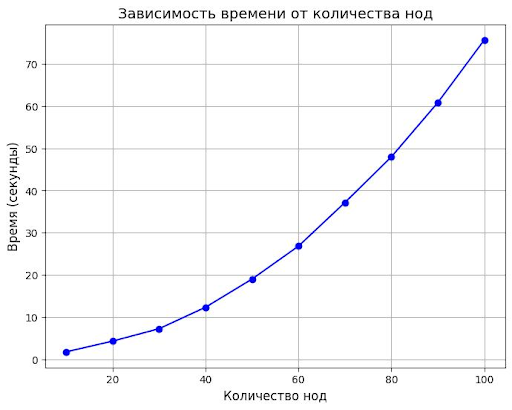
\includegraphics[width=0.9\linewidth]{figures/dijkstra.png}
    \end{center}

    \vspace{0.8cm}
    {\large \textbf{Неграфовые задачи}}
    \vspace{0.5cm}

    Также рассмотрено применение к неграфовым задачам на примере задачи SAT. Мы использовали сведение этой задачи к задаче поиска максимального независимого множества. Эту задачу мы решали рандомизированным алгоритмом Луби.
    \vspace{0.5cm}

    \begin{center}
      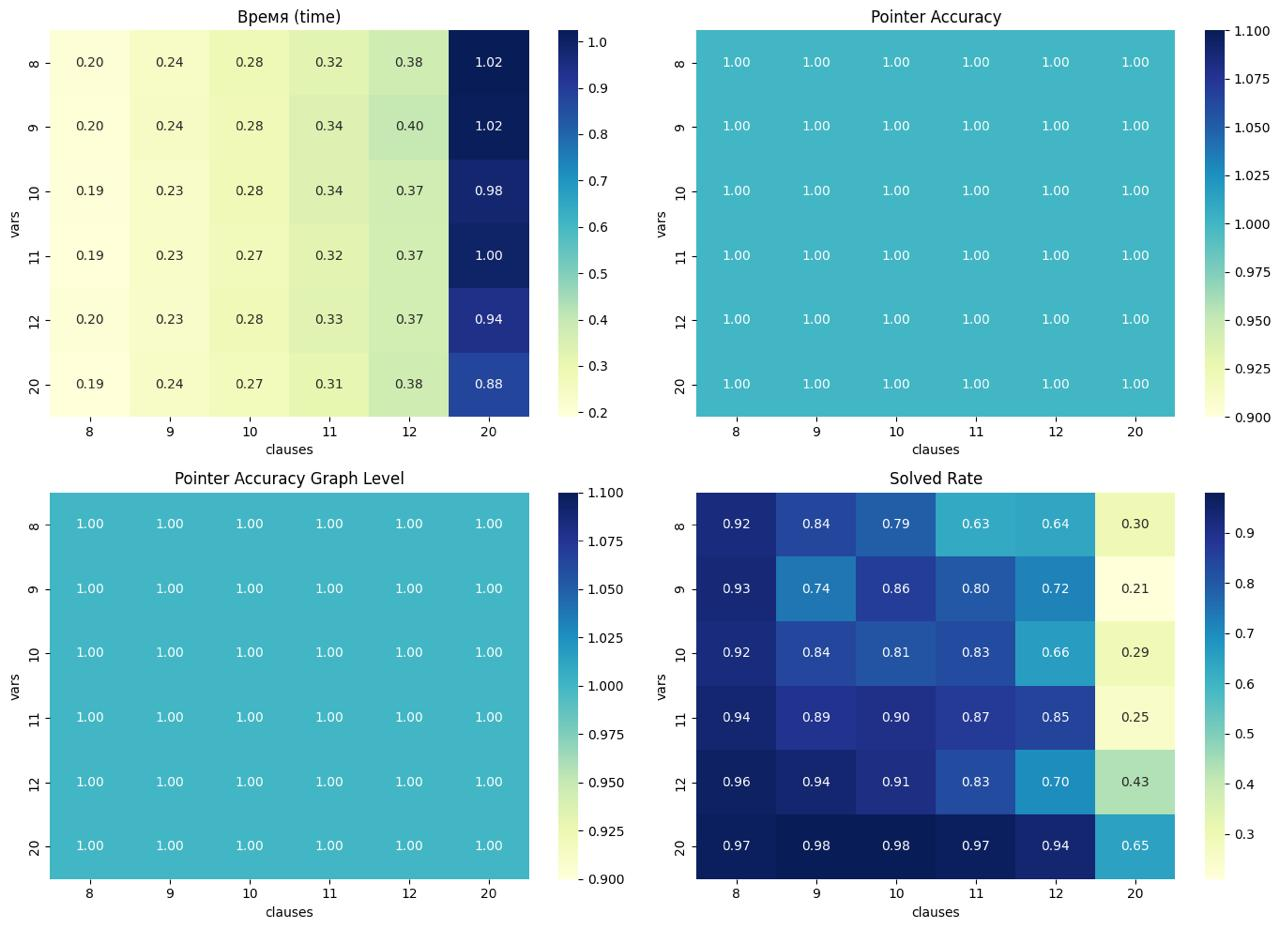
\includegraphics[width=\linewidth]{figures/sat.png}
    \end{center}
  \end{block}
  
  \begin{block}{Репозитории и исходный код}
\vspace{1em}

\begin{center}
    \begin{tabular}{c @{\hspace{0.15\linewidth}} c}
        
        % --- ЛЕВЫЙ QR-КОД ---
        \begin{minipage}{0.35\linewidth}
            \centering
            {\textbf{\textsf{DNAR + MILP}}} \\[0.8em]
            
\includegraphics[width=60mm, height=60mm]{images/qr-code-2.png}
        \end{minipage}
        &
        % --- ПРАВЫЙ QR-КОД ---
        \begin{minipage}{0.35\linewidth}
            \centering
            {\textbf{\textsf{AutoSAT}}} \\[0.8em]
            
\includegraphics[width=60mm, height=60mm]{images/qr-code.png}
        \end{minipage}

    \end{tabular}
\end{center}

\vspace{1em}
\end{block}

\end{column}

\separatorcolumn

% --- КОЛОНКА 2 ---
\begin{column}{\colwidth}


  \begin{block}{Оптимизация по времени}
    В контексте задач дискретной оптимизации важно оптимизировать время работы. Поэтому мы реализовали версию архитектуры, в котором квадратичный Attention был заменен линейной Mamba \cite{gu2024mambalineartimesequencemodeling}. Добились улучшения по временни, которое особенно заметно на задачах больших размерностях.

    \begin{center}
      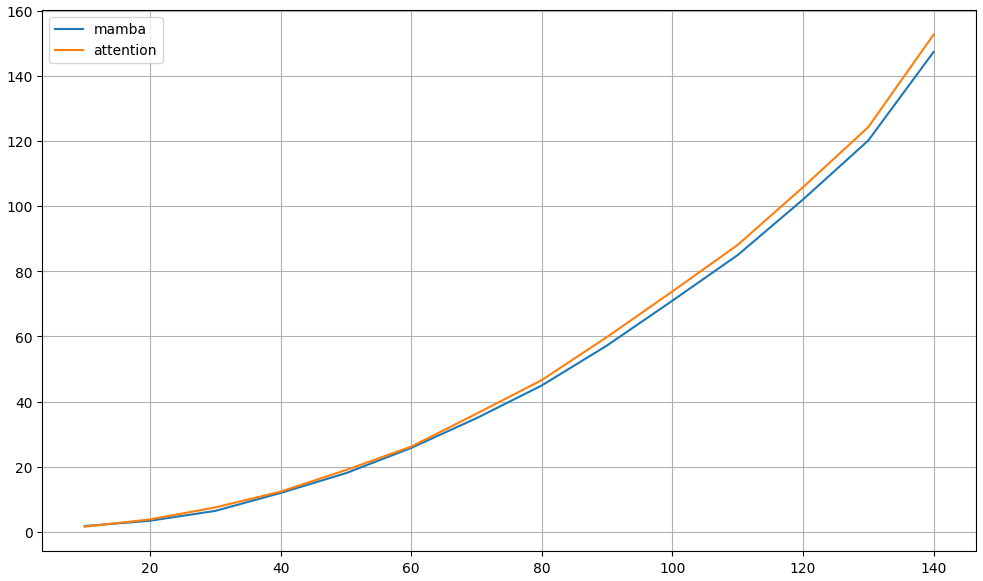
\includegraphics[width=0.9\linewidth]{figures/mamba_small.png}
    \end{center}
    \vspace{0.6cm}

    \begin{center}
      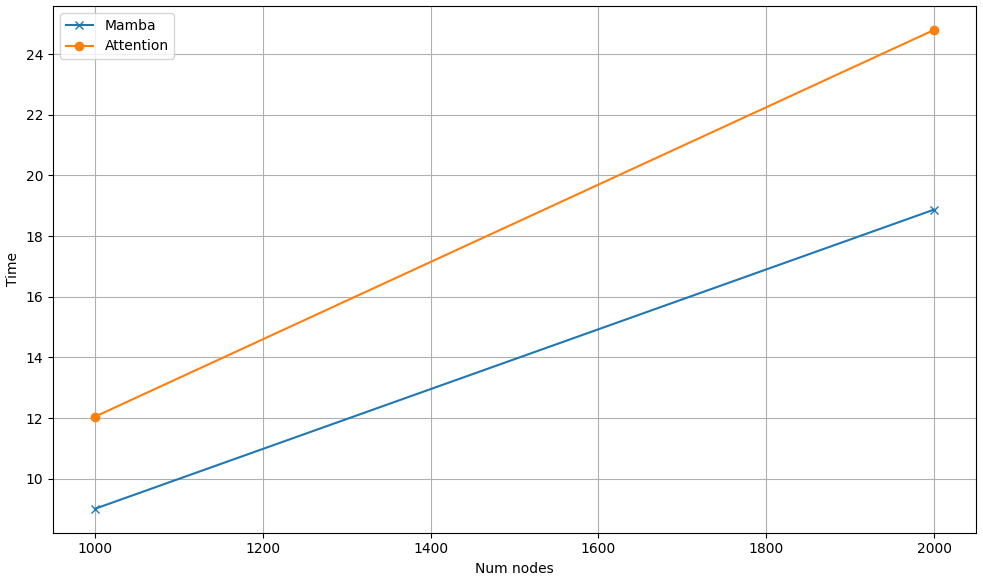
\includegraphics[width=0.925\linewidth]{figures/mamba_large.png}
    \end{center}
  \end{block}

    \begin{block}{Mixed integer linear programming problem}
    Рассмотрено применение к задаче MILP. Была рассмотрена версия алгоритма Branch\&Bound \cite{huang2021branchboundmixedinteger} с одновременным использованием стратегий Depth-first search и ветвления по `наиболее дробной` переменной. Без добавления шагов LP-солвера (релаксация к которому является частью этого алгоритма) в обучающий датасет, архитектура не продемонстрировала способность к обучению. \\
  
    Удалось применить архитектуру для выбора переменной ветвления в комбинации с внешним lp-солвером в роли оракула. Преимуществ по сравнению с обычным подходом такая комбинация не представляет (сравнение по времени на случайных задачах показано на графике). Однако остаётся возможность для обобщения архитектурой большого множества известных эвристик для Branch\&Bound (например применение наиболее оптимальной эвристики в зависимости от задачи) -- данная часть в процессе исследования. Также есть возможность использования архитектуры как первого приближения решения задачи.\\
    \begin{figure}[H]
        \centering
    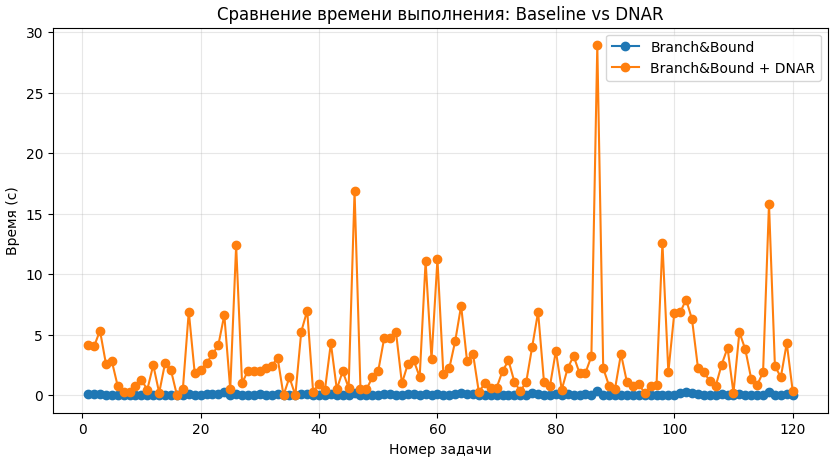
\includegraphics[width=\linewidth]{figures/milp.png}
    \end{figure}
  \end{block}

\begin{center}
      
\includegraphics[width=0.8\linewidth]{images/images.jpeg}
    \end{center}

  
\end{column}

\separatorcolumn

% --- КОЛОНКА 3 ---
\begin{column}{\colwidth}

  \begin{block}{AutoSAT}
    Алгоритм итеративно оптимизирует эвристики солвера. После каждой итерации LLM получает фидбэк о предложенной ею эвристике: как изменилось время работы солвера после смены эвристики на новую. Показано, что несмотря на значимые улучшений на тренировочной выборке, предложенные моделями эвристики нерелевантны вне тренировочной выборки.
  \end{block}

  \begin{block}{Таблица результатов}
    \begin{table}
      \centering
      \begin{tabular}{l r r c}
        \toprule
        \textbf{LLM} & \textbf{Temperature} & \textbf{Train diff} $\downarrow$ & \textbf{Eval diff} $\downarrow$ \\
        \midrule
        DeepSeek v3.1 & 0.9 &  -27\% & +4\%\\
        DeepSeek v3.1 & 0.8 & -8\% & +3\% \\
        DeepSeek v3.1 & 0.6 & -20\% & +3\% \\
        gpt-oss-120b & 0.9 & -15\%& +4\%\\
        gpt-oss-120b & 0.6 & -17\% & +7\%\\
        \bottomrule
      \end{tabular}
      \caption{Сравнение лучших результатов, показанных различными моделями}
    \end{table}
  \end{block}

\begin{block}{Изменение эвристики с помощью LLM}
\vspace{0.5em}

\footnotesize\ttfamily
\begin{tabular}{@{} p{0.48\linewidth} | p{0.48\linewidth} @{}}
\centering\textbf{\textsf{\textcolor{red}{Старый код}}} & \centering\textbf{\textsf{\textcolor{green!60!black}{Новый код}}} \tabularnewline
\hline
\vspace{0.2em}
void Solver::bump\_var(int var, double coeff) \{ \newline
\hspace*{2em}if ((activity[var] += var\_inc * coeff) > 1e100) \{ \newline
\hspace*{4em}for (int i = 1; i <= vars; i++) activity[i] *= 1e-100; \newline
\hspace*{4em}var\_inc *= 1e-100;\} \newline
\hspace*{2em}if (vsids.inHeap(var)) vsids.update(var); \newline
\}
&
\vspace{0.2em}
void Solver::bump\_var(int var, double coeff) \{ \newline
\hspace*{2em}double inc = var\_inc * coeff; \newline
\hspace*{2em}activity[var] += inc; \newline
\hspace*{2em}if (conflicts > 0) \{ \newline
\hspace*{4em}double conflict\_rate = (double)conflicts / (trail.size() + 1); \newline
\hspace*{4em}if (conflict\_rate > 0.05) \{ \newline
\hspace*{6em}inc *= 1.2; \newline
\hspace*{4em}\} \newline
\hspace*{2em}\} \newline
\hspace*{2em}if (level[var] > 0) \{ \newline
\hspace*{4em}double age\_factor = 1.0 / (1.0 + 0.01 * conflicts); \newline
\hspace*{4em}activity[var] *= age\_factor; \newline
\hspace*{2em}\} \newline
\hspace*{2em}if (activity[var] > 1e100) \{ \newline
\hspace*{4em}double scale = 1e-100; \newline
\hspace*{4em}for (int i = 1; i <= vars; i++) activity[i] *= scale; \newline
\hspace*{4em}var\_inc *= scale; \newline
\hspace*{2em}\} \newline
\hspace*{2em}if (vsids.inHeap(var)) vsids.update(var); \newline
\}
\tabularnewline
\end{tabular}

\end{block}

\begin{block}{Визуализация процесса обучения}
    \hfill
    \begin{columns}[t]
      \begin{column}{0.95\linewidth}
      
\includegraphics[width=\linewidth]{images/par2_vs_iter.png}
      \end{column}
    \end{columns}
\end{block}

  \begin{block}{Литература}
    \nocite{*} 
    \footnotesize
    \bibliographystyle{abbrv} 
    \bibliography{poster}     
  \end{block}

\end{column}

\separatorcolumn
\end{columns}
\end{frame}

\end{document}